\chapter{Estimating the Gap}\label{ch:estimation}

Chapter~\ref{ch:routeA} turned the gap into a property of a positive measure. This chapter treats it as a parameter to be estimated from data, which is how lattice gauge theory meets it in practice. The main point is simple and underused: the spectral measure\index{spectral measure} itself is poorly determined by a noisy correlator, but the left edge of its support is well determined. The first sections develop the support constrained profile estimator and test it on a toy spectrum. The remaining three sections treat Monte Carlo methods from Bayesian computation that bear on estimation in lattice gauge theory: latent variable samplers and nested sampling (Section~\ref{ch:latent}), the vertical likelihood and split sampling (Section~\ref{ch:vertical}), and weighted Monte Carlo with the Yakowitz rate (Section~\ref{ch:yakowitz}).

\section{The inverse Laplace problem}

A lattice simulation produces estimates $y_i$ of $C(\tau_i)$ at a finite set of Euclidean times, with a covariance matrix estimated from the Monte Carlo samples. Recovering $\mu$ from $y$ means inverting the Laplace transform, one of the most ill conditioned problems in applied mathematics. The singular values of the Laplace operator restricted to a finite interval decay geometrically, so information about $\mu$ at fine resolution is lost exponentially fast in the noise. Very different measures can have Laplace transforms that agree to within any reasonable statistical error on a finite window.

In lattice QCD the problem goes by the name of spectral reconstruction, and the standard methods are the Backus Gilbert method~\cite{BG68}, maximum entropy, and the smeared spectral density approach of Hansen, Lupo and Tantalo \cite{HLT}, which targets $\mu$ convolved with a chosen kernel rather than $\mu$ itself. All of these accept that $\mu$ cannot be resolved pointwise.

\section{Positivity as the prior}

The Thorin viewpoint suggests a different emphasis. We know two things about $\mu$ with certainty: it is nonnegative, and it is supported on $[\Delta,\infty)$. The first is a constraint; the second is the quantity of interest. This is exactly the setting of positive linear inverse problems.

\begin{definition}
Given a grid $E_1<\dots<E_J$ and the kernel $K_{ij}=e^{-\tau_iE_j}$, the positive deconvolution\index{positive deconvolution} problem is to find $\nu\in[0,\infty)^J$ with $K\nu\approx y$.
\end{definition}

Vardi and Lee\index{Vardi, Y.!and Lee, D.}'s EM algorithm \cite{VL},
\[
\nu_j\leftarrow\nu_j\,\frac{\sum_iK_{ij}\,y_i/(K\nu)_i}{\sum_iK_{ij}},
\]
keeps $\nu$ positive at every step and decreases a Kullback Leibler divergence. Polson and Robert \cite{PR} interpreted the same iteration as a Monte Carlo inversion in the spirit of von Neumann, which opens the door to sampling based uncertainty quantification. Padilla, Polson and Scott \cite{PPS} give a Bayesian nonparametric treatment of deconvolution with guarantees on posterior contraction, and proximal methods, surveyed by Polson, Scott and Willard \cite{PSW15}, accelerate the fitting.

\section{The support constrained profile}

The new ingredient is to treat the gap as an explicit parameter.

\begin{definition}
For a candidate gap $\delta$, let
\[
\chi^2(\delta)=\min\Big\{(y-K\nu)^\top\Sigma^{-1}(y-K\nu):\ \nu\ge0,\ \nu_j=0\text{ for }E_j<\delta\Big\}.
\]
\end{definition}

The function $\chi^2(\delta)$ is nondecreasing in $\delta$, since raising $\delta$ shrinks the feasible set. As long as $\delta$ is below the true gap, the constrained fit can match the data as well as the unconstrained one. As soon as $\delta$ passes the true gap, the fit must replace the lightest state by heavier ones, whose Laplace transforms decay faster, and the misfit at large $\tau$ grows sharply. A natural estimate is
\[
\hat\Delta=\min\{\delta:\chi^2(\delta)-\chi^2_{\min}>c\}
\]
for a threshold $c$, with $c=4$ a convenient default. Each $\chi^2(\delta)$ is a nonnegative least squares problem, solved exactly by the Lawson and Hanson~\cite{LH74} algorithm.

\section{A worked example}

We used the toy spectrum of Chapter~\ref{ch:routeA}: stable states at $E=1,1.5,1.9$ with weights $1,0.6,0.3$, and a two particle continuum from $E=2$ with density $0.4\sqrt{E-2}\,e^{-0.3(E-2)}$. The correlation was computed at $\tau=0.1,0.2,\dots,6$, and independent Gaussian noise with standard deviation $0.2\%$ of each value was added.

Figure~\ref{fig:deconvB} shows the result. On the left, the EM reconstruction smears the three atoms into a broad bump, as any inverse Laplace method must at this noise level. On the right, the profile $\chi^2(\delta)$ is flat for $\delta<1$ and rises by many orders of magnitude just past $\delta=1$. The estimate is $\hat\Delta=1.02$, on a candidate grid with spacing $0.02$ (the table below uses spacing $0.01$).

\begin{figure}[t]
\centering
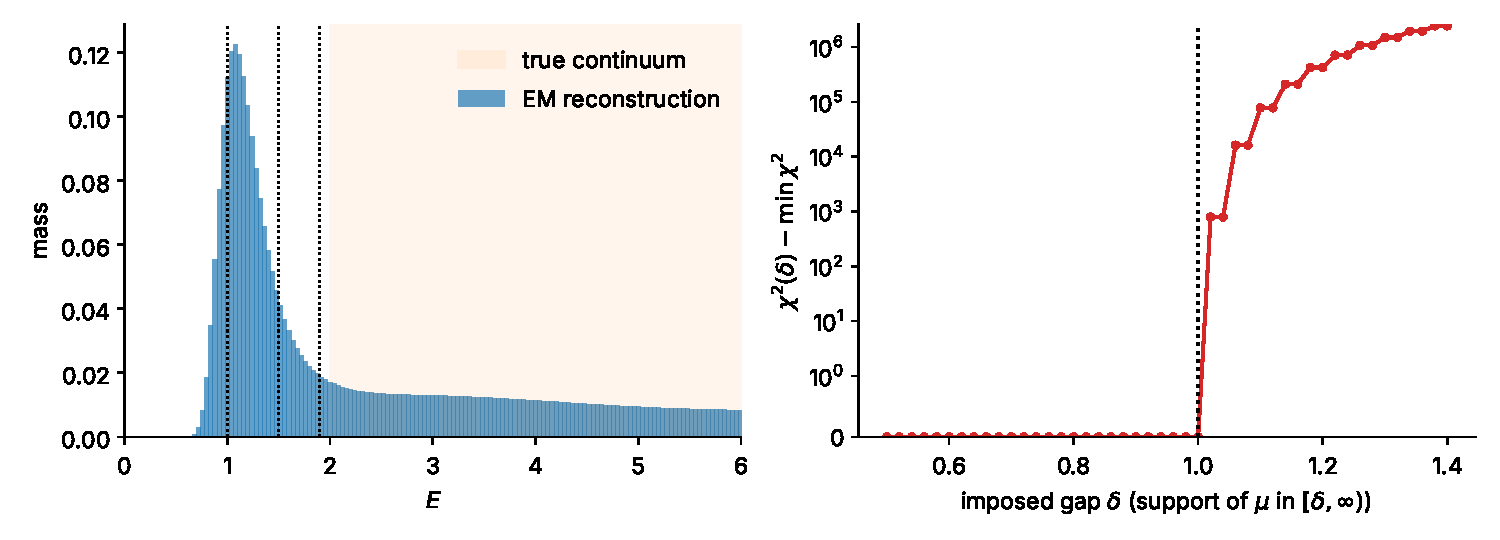
\includegraphics[width=\textwidth]{figures/deconvolution_gap.pdf}
\caption[Left: Vardi and Lee EM reconstruction of the spectral measure from a noisy correlator; dotted lines]{Left: Vardi and Lee EM reconstruction of the spectral measure from a noisy correlator; dotted lines mark the true atoms. Right: the support constrained profile $\chi^2(\delta)$ locates the gap sharply even though the measure itself is smeared.}
\label{fig:deconvB}
\end{figure}

Repeating the experiment twenty times at each noise level gave the following estimates, on a grid of candidate gaps with spacing $0.01$ and an energy grid with spacing $0.04$ (script \texttt{code/gap\_noise\_table.py}).
\begin{center}
\begin{tabular}{rccc}
\toprule
relative noise & mean $\hat\Delta$ & standard deviation & range \\ \midrule
0.1\% & 1.010 & 0.000 & 1.010 \\
0.5\% & 1.010 & 0.000 & 1.010 \\
1.0\% & 1.010 & 0.000 & 1.010 \\
2.0\% & 1.016 & 0.014 & 1.010 to 1.050 \\
\bottomrule
\end{tabular}
\end{center}
The estimate is pinned at the first candidate above the energy grid point $E=1$ up to one percent noise, so in this experiment the energy grid, not the noise, limits the resolution. At two percent noise the estimate begins to drift upward. Noise can only delay the rejection of a candidate above the true gap, so the estimate errs on the side of a larger gap, in line with the general lesson that data bound the gap from above.

\section{A Bayesian formulation}

The profile is the frequentist face of a simple hierarchical model. Put a prior $\pi(\delta)$ on the gap, and given $\delta$ a prior on positive measures supported on $[\delta,\infty)$, for instance a gamma process or a finite mixture with a sparsity prior on the weights. The likelihood is Gaussian in $y$. The marginal posterior of $\delta$ integrates the measure out, and EM or a proximal algorithm computes the conditional mode of the measure at each $\delta$. A Laplace approximation to the integral gives
\[
\log p(\delta\mid y)\approx-\tfrac12\chi^2(\delta)+\log\pi(\delta)+\log p(\hat\nu_\delta\mid\delta)+\tfrac{d_\delta}{2}\log2\pi-\tfrac12\log\det\mathcal I(\delta)+\text{const},
\]
where $\hat\nu_\delta$ is the constrained fit, $d_\delta$ the number of its nonzero components, and $\mathcal I(\delta)$ the observed information on them. Horseshoe type priors~\cite{CPS10} on the weights, which shrink small atoms hard while leaving large ones alone, are natural here: the spectrum of a gauge theory has a few stable states and a continuum, which is a sparse signal plus a smooth background.

\section{What estimation can and cannot do}

Local rates and the profile estimate both err toward a larger gap, so data bound the gap from above. Estimation can expose a wrong claim about the spectrum and measure a lattice gap precisely; it cannot prove that a gap exists or reach the continuum. Its role for the Clay problem is diagnostic: any proof strategy predicts lattice gaps at intermediate couplings, and those predictions can be tested with the methods of this chapter. The Migdal Kadanoff ladder of Section~\ref{ch:mk} makes such predictions.

\section{Latent Variables and Nested Sampling}\label{ch:latent}

Two families of Monte Carlo methods from Bayesian computation bear directly on lattice gauge theory: latent variable (auxiliary variable) Markov chain Monte Carlo, in the line of Swendsen and Wang\index{Swendsen, R. H.!and Wang, J. S.} \cite{SW87}, Edwards and Sokal \cite{ES88}, Besag and Green \cite{BG93}, and Higdon\index{Higdon, D.} \cite{Hi98}, together with slice sampling\index{slice sampling}, the Birge and Polson optimisation by slice sampling \cite{BP}, and Polson's 1996 embedding of a Cauchy likelihood in a log concave posterior \cite{Po96}; and Skilling's nested sampling\index{nested sampling} \cite{Sk06}, which Murray, MacKay, Ghahramani and Skilling applied to Potts models \cite{MMGS}. This section asks whether they are useful for the mass gap. The answer is yes in two ways and possibly in a third: as samplers for the lattice measures from which gaps are estimated, as a way of computing partition functions at every coupling at once, and, possibly, as a source of the common probability space that the comparison problem of Chapter~\ref{ch:path} needs.

\subsection{The heat bath is a latent variable method}

For SU(2), write a link as a unit quaternion $U\in S^3$. With all other links fixed, the Wilson action depends on $U$ only through the sum $A$ of the staples that complete its plaquettes (six in four dimensions, two in two), and a sum of SU(2) elements is a nonnegative multiple of an SU(2) element, $A=kV$. The conditional law of $U$ is therefore
\[
p(U\mid\text{rest})\propto\exp\big(\beta k\,\langle U,V^{-1}\rangle\big),
\]
a von Mises Fisher\index{von Mises Fisher law} law on $S^3$ with mean direction $V^{-1}$ and concentration $\beta k$. Creutz's heat bath \cite{Cr80} samples it exactly: writing $UV=a_0+i\sum_{j=1}^3a_j\sigma_j$, the component $a_0$ has density proportional to $\sqrt{1-a_0^2}\,e^{\beta ka_0}$ on $[-1,1]$, and the remaining direction is uniform on a two sphere.

Slice sampling makes the latent structure explicit. Introduce $u\mid a_0\sim\mathrm{Uniform}(0,e^{\beta ka_0})$. Then $a_0\mid u$ is distributed as $\sqrt{1-a_0^2}$ restricted to $a_0>\log u/(\beta k)$, which is easy to sample. The Kennedy and Pendleton algorithm \cite{KP85}, the standard SU(2) heat bath at weak coupling, is a rejection scheme of the same kind. These are instances of Higdon's general auxiliary variable framework, in which a latent variable makes the conditional of the original variable simple. Polson's 1996 construction, embedding a heavy tailed Cauchy likelihood in a log concave posterior through latent scale variables, is the same device used to restore log concavity.

\subsection{Swendsen and Wang, Edwards and Sokal, and partial decoupling\index{partial decoupling}}

For the Ising and Potts models the decisive latent variable method is the Swendsen and Wang algorithm. Each bond receives a latent indicator that is switched on with probability $1-e^{-\beta}$ when its two spins agree (the Potts convention, with weight $e^{\beta\delta_{\sigma_i\sigma_j}}$); given the bonds, clusters of connected spins are recoloured independently. Edwards and Sokal identified the joint law of spins and bonds, whose bond marginal is the Fortuin and Kasteleyn~\cite{FK72} random cluster model. The method reduces critical slowing down because a single update can flip clusters of any size.

Higdon's 1998 paper generalised this to partial decoupling: the latent bonds absorb only a fraction of each interaction, so that clusters are smaller but the remaining interactions keep the image model faithful. Partial decoupling trades mixing speed against fidelity in a controlled way, and it applies to models, like spatial image priors, for which full decoupling gives clusters that are too large to be useful.

For gauge theories the picture is less favourable. Cluster constructions have been proposed for $\Z_2$ lattice gauge theory and some abelian models, but we know of no efficient cluster algorithm for SU(N) lattice gauge theory. The obstruction is the one met throughout this book: no Fortuin Kasteleyn representation is known with the monotonicity that makes clusters percolate in step with the physics, and no FKG inequality is known for nonabelian link variables. Partial decoupling in Higdon's sense remains a plausible way to reduce autocorrelations, for example by decoupling the abelian part of each plaquette interaction, but we do not know of a version for SU(N) that has been shown to help.

\subsection{The character expansion as a latent variable model}

There is a second, exact latent variable representation of every lattice gauge theory, and it connects directly to positivity. Expand each plaquette weight in characters, $f(U_p)=\sum_nn\,c_n\chi_n(U_p)$, and introduce a latent label $n_p$ for each plaquette. The joint weight of links and labels is
\[
\prod_p n_p\,c_{n_p}\,\chi_{n_p}(U_p).
\]
Integrating out the links with Haar measure forces the labelled plaquettes to form closed surfaces with compatible labels, giving a sum over decorated surfaces; this is the strong coupling expansion of Chapter~\ref{ch:strong}, and the surface sums studied by Chatterjee \cite{Ch19so,Ch19} and others. The label weights $n_pc_{n_p}$ are nonnegative exactly when $c_n\ge0$, which is the Osterwalder Seiler~\cite{OSe} sufficient condition for reflection positivity (Chapter~\ref{ch:positivity}). The characters $\chi_{n_p}(U_p)$ change sign, so the joint weight of links and labels is not itself nonnegative: the positivity is that of the label factors, and we do not claim that reflection positivity implies a positive latent representation.

Two consequences matter here. First, the Migdal Kadanoff step acts on the latent weights in a simple way: decimation raises the normalised coefficients $c_n$ (the label weights up to the factor $n$) to the power $b^2$, and bond moving combines labels by the Clebsch Gordan rule with nonnegative multiplicities (Lemma~\ref{lem:posB}). The renormalization ladder is a flow on the label weights, which are nonnegative when $c_n\ge0$. Second, worm and surface algorithms that sample the labels directly can be read as the dual, latent side of a Swendsen and Wang type scheme.

\subsection{Nested sampling}

Nested sampling, introduced by Skilling, computes the evidence $Z=\int L(x)\,\pi(\mathrm dx)$ by compressing the prior mass. It keeps $N$ live points drawn from the prior subject to $L>L^*$, repeatedly discards the point with the lowest likelihood, raises the threshold $L^*$ to its value, and replaces it by a new point drawn from the prior subject to the new threshold. After $i$ steps the prior mass $X_i$ above the threshold satisfies $\E\log X_i=-i/N$, and
\[
Z\approx\sum_i(X_{i-1}-X_i)\,L_i .
\]
The shrinkage factors $X_i/X_{i-1}$ are independent Beta$(N,1)$ variables, so $-\log X_i$ is a sum of independent exponential variables with mean $1/N$: the compression is a Poisson process in $-\log X$. Nested sampling is thus a first passage construction of the same kind as the renormalization walk of Section~\ref{ch:verification}, with the likelihood threshold playing the role of the coupling.

Murray, MacKay, Ghahramani and Skilling applied nested sampling to Potts models and showed two things that matter for gauge theory. Because the sampler works with likelihood contours rather than temperatures, it is not trapped by first order phase transitions, where thermodynamic integration and tempering fail. And one run gives the partition function at every temperature, since the dead points and their prior masses estimate the whole density of states\index{density of states}. Polson and Scott's vertical likelihood Monte Carlo \cite{PSvl} makes the same idea, integrating over likelihood levels rather than parameter space, the basis of a general estimator (Section~\ref{ch:vertical}).

\subsection{The density of states and Bernstein in the coupling}

For SU(2) lattice gauge theory take the prior to be the Haar measure on all links and the likelihood $e^{-\beta S}$ with $S=\sum_p(1-\frac12\operatorname{tr}U_p)\ge0$. Nested sampling records the action thresholds $S_i$ and prior masses $X_i$, which estimate the density of states $\rho$ of the action under Haar measure, and then
\[
Z(\beta)=\int_0^\infty e^{-\beta S}\,\rho(S)\,\mathrm dS
\]
for every $\beta$ at once. This formula is a Laplace transform of a nonnegative measure, so $Z$ is completely monotone in the coupling. The spectral measure of Chapters~\ref{ch:positivity} and~\ref{ch:routeA}, a measure on energies indexed by Euclidean time, has a counterpart here, a measure on actions indexed by the coupling, and complete monotonicity, the starting point of the Thorin machinery, holds for it. Its support reaches down to $S=0$, the pure gauge configurations, so there is no gap in $\beta$: as in the massless example of Section~\ref{ch:examples}, $Z(\beta)$ decays polynomially as $\beta\to\infty$, with an exponent set by the number of fluctuating modes. Density of states methods are established in lattice gauge theory, for example the linear logarithmic relaxation method of Langfeld, Lucini and Rago \cite{LLR}; nested sampling is a Bayesian route to the same object, with built in error estimates.

\subsection{A test with an exact answer}

Two dimensional lattice gauge theory gives an exact check. On an $m\times m$ torus with $P=m^2$ plaquettes and Haar normalised links, the character expansion gives
\[
Z(\beta)=e^{-\beta P}\sum_{n\ge1}c_n(\beta)^P,\qquad c_n(\beta)=\frac{2I_n(\beta)}{\beta},
\]
because the torus has Euler characteristic zero. We ran nested sampling for SU(2) on a $3\times3$ torus, with $200$ live points and replacement by a constrained random walk on single links with adaptive step size, for $6490$ iterations, until the action threshold fell to $0.6$, a compression of the prior by a factor $e^{-32.5}$. A plain Monte Carlo average over $20{,}000$ Haar configurations at $\beta=1$ gives $\log Z(1)=-7.8970$ against the exact $-7.8975$, confirming the formula.

\begin{figure}[t]
\centering
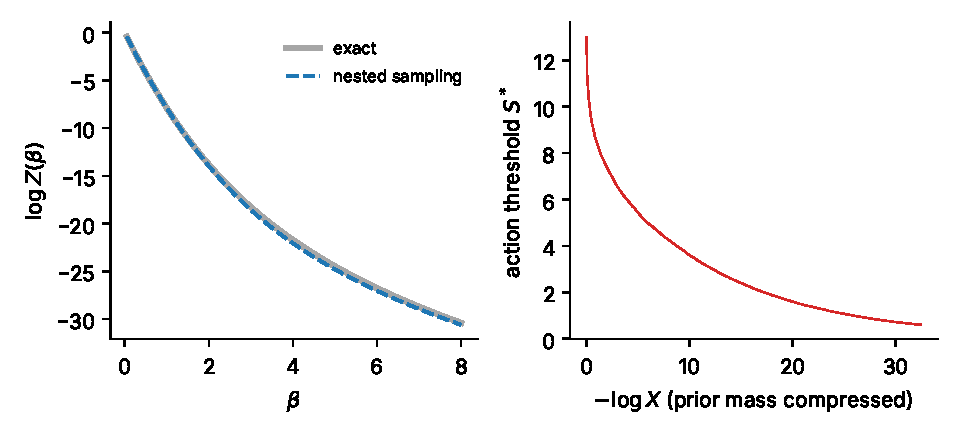
\includegraphics[width=\textwidth]{figures/nested_su2.pdf}
\caption[Nested sampling for two dimensional SU(2) on a $3\times3$ torus]{Nested sampling for two dimensional SU(2) lattice gauge theory on a $3\times3$ torus. Left: $\log Z(\beta)$ from a single run, against the exact character formula, for all $\beta$ in $[0.05,8]$. Right: the action threshold against the compression $-\log X$; it is the inverse cumulative density of states of the action under Haar measure.}
\label{fig:nested}
\end{figure}

The single run reproduces $\log Z(\beta)$ over the whole range $\beta\in[0.05,8]$ (Figure~\ref{fig:nested}; script \texttt{code/nested\_su2.py}), with largest error $0.35$, near $\beta\approx4$ ($0.20$ at $\beta=8$). That is the size expected from Skilling's estimate \cite{Sk06} $\sqrt{H/N}$ of the standard error of $\log Z$, since reaching the posterior at $\beta=8$ requires an information $H$ of about eighteen nats; more live points shrink it at the usual Monte Carlo rate. The test is small, but it shows the two features that matter: one run serves all couplings, and the output is a positive measure whose Laplace transform is the partition function.

\subsection{Are these methods useful for the mass gap?}

For estimation, yes. Measuring lattice gaps near the continuum limit is limited by autocorrelation, and in four dimensions above all by the freezing of topological charge as the lattice spacing shrinks. Methods that move along likelihood contours, such as nested sampling, or that act on large latent structures, such as cluster and worm algorithms, are the natural candidates for multimodal and slowly mixing targets. The support constrained gap estimator of this chapter needs correlators at large Euclidean times, which is where better samplers pay off.

For the renormalization ladder, yes. The heat kernel projection of Section~\ref{ch:verification} replaces each effective plaquette law by a one parameter family. Nested sampling on a single Migdal Kadanoff block, or on a small block of the true lattice, computes the full effective partition function as a function of the coupling, which is the input needed to test the projection, to follow the flow without truncation, and to compare the Migdal Kadanoff block with a true block.

For the proof, possibly, and this is the most interesting point. The comparison problem of Chapter~\ref{ch:path} asks for a true block spin step and a Migdal Kadanoff step on a common probability space, compared in the likelihood ratio order. Latent variable constructions are exactly how such common spaces are built. The monotonicity of the random cluster model (the FKG and comparison inequalities) belongs to the model of Fortuin and Kasteleyn itself, and the Edwards and Sokal joint representation is what carries the random cluster results, including coupling proofs of exponential decay, over to the Potts model. Higdon's partial decoupling interpolates between the original model and a decoupled one, which is the kind of interpolation a sandwich needs. The label weights of the character expansion are nonnegative when $c_n\ge0$, which supplies positivity for the label factors only. What it does not supply is a monotone coupling: without an FKG inequality for nonabelian link variables, the clusters or surfaces of one theory need not dominate those of the other. Finding a latent representation of SU(N) gauge theory with the right monotonicity, perhaps one built from the Biane Pitman Yor variables \cite{BPY} that carry the curvature, would be a genuine step on the open problem of Chapter~\ref{ch:path}.

\section{Vertical Likelihood and Split Sampling}\label{ch:vertical}\index{vertical likelihood}\index{split sampling}\index{Polson, N. G.!and Scott, J. G.}

The partition function of a lattice gauge theory is a normalising constant. Every method for computing normalising constants in Bayesian statistics therefore has a lattice counterpart, and the vertical likelihood perspective of Polson and Scott \cite{PSvl} organises the most important of them under one principle. This section lists the methods it unifies, adds split sampling, implements all of them on a lattice gauge theory with an exact answer, and asks which are useful for the mass gap.

\subsection{The vertical representation}

Let $\pi$ be a probability measure, the prior, and $L\ge0$ a likelihood, with $Z=\int L\,\mathrm d\pi$. Polson and Scott build everything from two functions: the upper tail function of the likelihood ordinate,
\[
T(y)=\pi\{x:L(x)>y\},
\]
the prior mass above level $y$, and its pseudo inverse $\ell(s)=\sup\{y:T(y)>s\}$. Interchanging the order of integration gives two one dimensional identities,
\[
Z=\int_0^\infty T(y)\,\mathrm dy=\int_0^1\ell(s)\,\mathrm ds .
\]
The integral over the original space, of any dimension, collapses onto the line of likelihood ordinates. This is the vertical view: instead of integrating across the space horizontally, integrate up the likelihood.

For lattice gauge theory the prior is Haar measure on the links, the likelihood is $e^{-\beta S}$, and the level sets $\{L>y\}$ are the action sublevel sets $\{S<s\}$. Then $T(y)$ is the prior mass $X(s)$ of configurations with action below $s$, the cumulative density of states, and
\[
Z(\beta)=\int_0^\infty e^{-\beta s}\,\mathrm dX(s),
\]
the Laplace transform in the coupling of the density of states introduced in Section~\ref{ch:latent}.

\subsection{The vertical likelihood principle}

The one dimensional identities are not to be used by direct quadrature: $T(y)$ changes far too quickly near the top of the likelihood. Polson and Scott use them instead to design importance functions. Choose a weight function $w\ge0$ on likelihood ordinates with cumulative $W(u)=\int_0^uw$ (where $w$ may carry an atom at $0$, so that $W(0)>0$), and form the joint law
\[
\pi_w(x,u)\propto w(u)\,\mathrm{I}\{0<u<L(x)\}\,\pi(x),
\]
whose $x$ marginal is $\pi_w(x)\propto\pi(x)W(L(x))$. Sampling $x$ from $\pi_w$ and taking the ratio of the means of $L/W$ and $1/W$ estimates $Z$. The design problem, which in ordinary importance sampling is the choice of a proposal over a high dimensional space, is reduced to the choice of a one dimensional weight function on the likelihood ordinate.

\begin{theorem}[Polson and Scott \cite{PSvl}]
If $T(y)$ is differentiable and $\xi\sim\pi_w$, the likelihood ordinate $Y=L(\xi)$ has density $f(y)=-W(y)T'(y)/Z_w$, where $Z_w=\int W(L)\,\mathrm d\pi$.
\end{theorem}
\begin{proof}
Under $\pi$ the ordinate $Y=L(\xi)$ has survival function $T(y)$, hence density $-T'(y)$. The $x$ marginal $\pi_w$ reweights $\pi$ by $W(L(x))/Z_w$, so the ordinate density is $W(y)(-T'(y))/Z_w$.
\end{proof}

The score function heuristic asks that the ordinate density be proportional to $-T'(y)/T(y)$, concentrating samples where the tail function changes fastest relative to its size, since that is where the integral $\int T(y)\mathrm dy$ is decided. The theorem then says to take $W(u)=1/T(u)$, and the default weight is the truncated version
\[
W(u)=\frac{1}{\max\{\eta,T(u)\}},\qquad 0<\eta\le1 .
\]
Sampling from $\pi_w$ is done by weighted slice sampling, alternating $u\mid x$ from $w$ truncated to $(0,L(x))$ and $x\mid u$ from the prior truncated to $\{L(x)>u\}$.

\subsection{The methods it unifies}

Polson and Scott \cite{PSvl} show that seven classes of methods are special cases or close relatives, distinguished by the weight function.
\begin{enumerate}
\item Importance sampling, with any proposal, implies some law of the ordinate; the vertical view chooses that law directly.
\item Slice sampling: the uniform weight $w\equiv1$ recovers the ordinary slice sampler conditionals, whose target is the posterior.
\item Annealing and tempering: $w(u)=au^{a-1}$ gives $W(u)=u^a$ and the power posterior $p\,L^a$ of Friel and Pettitt~\cite{FP08}, the basis of simulated and annealed importance sampling; adding a point mass at zero gives bridge and path sampling.
\item The harmonic mean estimator: with $w\equiv1$ the weights are $1/L$, which is the Newton and Raftery~\cite{NR94} estimator, with its well documented infinite variance.
\item Troutt's vertical density sampler~\cite{Tr91}, of which the theorem above is a generalisation.
\item Energy level sampling from statistical physics: $W=1/\rho(s)$, with $\rho$ the density of states of Section~\ref{ch:latent}, gives multicanonical sampling and the Wang and Landau~\cite{WL01} algorithm, and $W=1/X(s)$, the untruncated default weight, the $1/k$ ensemble of Hesselbo and Stinchcombe~\cite{HS95}.
\item Nested sampling, which Polson and Scott show sequentially constructs an importance function close to the default score function weight.
\end{enumerate}

\subsection{Split sampling and optimisation by slicing}

Split sampling, which we take from unpublished work of Birge, Chang and Polson, estimates expectations and rare event probabilities in high dimensions. It splits the quantity of interest into an integrated family of normalisation constants indexed by an auxiliary level variable, runs an MCMC on the joint space of state and level, and adapts weights on the levels, in the manner of Wang and Landau, so that every level is visited. The marginal occupation of the levels then estimates the rare event probabilities $X(s_t)$ at the level values $s_t$, and the expectation is assembled from them. For likelihood level sets this is a discrete version of the vertical identity, with the levels chosen adaptively. Birge and Polson's optimisation by slice sampling \cite{BP} uses the same auxiliary variable construction to locate maxima: the slice variable pushes the chain up the likelihood, and in the limit of a sharpening weight it concentrates on the mode.

For gauge theory, both ideas fit naturally. The rare events are configurations of low action, or of nontrivial topology, which a standard Markov chain rarely visits at weak coupling. Split sampling across action levels or across topological sectors is a principled way to visit them, and optimisation by slicing locates the classical minima of the action, around which the weak coupling expansion is built.

\subsection{An implementation with an exact answer}

We implemented the methods on two dimensional SU(2) lattice gauge theory on a $3\times3$ torus, where $\log Z(2)=-13.8223$ exactly from the character formula of Section~\ref{ch:latent}. Each method received about $2.4\times10^5$ single link updates of its own (the harmonic mean about half that); the vertical likelihood sampler and split sampling also reuse the nested sampling run as a pilot, so their total cost is about twice that of the others. The posterior kernel throughout is the slice sampling heat bath of Section~\ref{ch:latent}, which reproduces the exact posterior mean action, $5.10$ at $\beta=2$, to within Monte Carlo error. The vertical likelihood sampler uses the default weight with $X(s)$ estimated by a pilot nested run, and split sampling uses thirteen action levels spaced evenly in $\log X$ down to $e^{-14}$, with Wang and Landau adaptation of the level weights. Three independent seeds (5, 11 and 23) give the following root mean square errors in $\log Z(2)$, each taken over the three seeds. The script \texttt{code/vl\_methods.py} saves the per seed results in \texttt{results/}, and \texttt{code/book\_figs4.py} builds the table and the figure from them.

\begin{center}
\footnotesize
\resizebox{\textwidth}{!}{\begin{tabular}{lcc}
\toprule
method & weight $W(u)$ & RMSE \\ \midrule
prior importance sampling & $1$ & 0.117 \\
harmonic mean & $u$ & 0.275 \\
power posterior path sampling & $u^a$ ladder & 0.057 \\
nested sampling & sequential, near $1/T(u)$ & 0.218 \\
vertical likelihood, Metropolis on $\pi_w$ & $1/\max\{\eta,T(u)\}$ & 0.032 \\
split sampling & adaptive on levels & 0.140 \\
Wang and Landau & $1/\rho(s)$ & not converged \\
\bottomrule
\end{tabular}}
\end{center}

\begin{figure}[t]
\centering
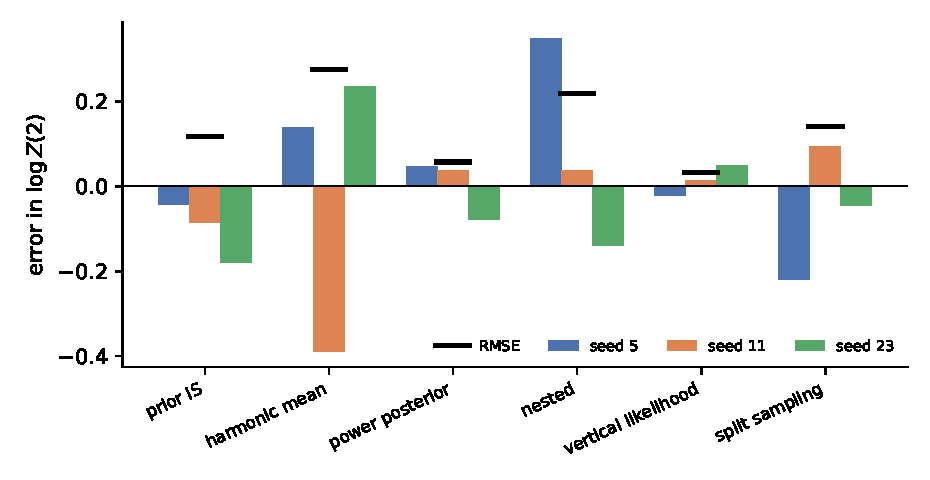
\includegraphics[width=\textwidth]{figures/vl_errors.pdf}
\caption[Errors of the vertical likelihood family on two dimensional SU(2)]{Errors in $\log Z(2)$ for five members of the vertical likelihood family and split sampling on the $3\times3$ SU(2) torus, three seeds each, with the root mean square error marked. The harmonic mean has the largest errors and no stable sign, as its infinite variance theory predicts.}
\label{fig:vlerrors}
\end{figure}

Three lessons stand out. First, the harmonic mean is the least accurate and its error changes sign between seeds ($+0.14$, $-0.39$, $+0.24$), as its infinite variance theory predicts. Second, the vertical likelihood sampler has the smallest error here ($0.032$), followed by power posterior path sampling ($0.057$), while plain importance sampling from the prior ($0.117$) is already competitive with split and nested sampling on this small problem with a modest likelihood. With three seeds the order of the closer methods is not established. Polson and Scott report that on sharper likelihoods, as in their fifty dimensional example, weighted slice sampling beats nested sampling by a wide margin \cite{PSvl}. Third, Wang and Landau did not converge within the common budget: the flat histogram condition was not met in the rarely visited energy bins, and anchoring an unconverged density of states produces large errors. Adaptive energy level methods need budgets far beyond those of the other methods.

\begin{figure}[t]
\centering
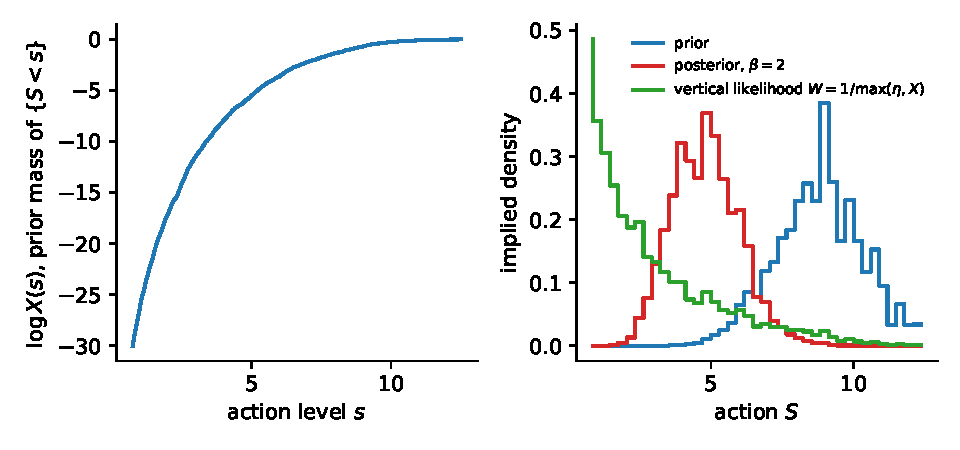
\includegraphics[width=\textwidth]{figures/vl_implied.pdf}
\caption[Implied laws of the action under three weight functions]{Left: the prior mass $X(s)$ of $\{S<s\}$ from a nested run, the cumulative density of states. Right: the implied law of the action under the prior, under the posterior at $\beta=2$, and under the default vertical likelihood weight, which spreads samples across all action levels.}
\label{fig:vlimplied}
\end{figure}

\subsection{Are vertical likelihood methods useful for the gap?}

Yes, for the reasons given for nested sampling in Section~\ref{ch:latent}, and for two more. The score function heuristic is the right principle for visiting the rare, low action configurations that dominate at weak coupling, and split sampling by topological sector would be a natural attack on topological freezing, though we did not test it (the two dimensional torus has no topological sectors). The methods are also diagnostics for the renormalization ladder: the partition function of a single block, as a function of the coupling, determines the Migdal Kadanoff step, and vertical methods compute it without truncating the character expansion.

\section{Weighted Monte Carlo and the Yakowitz Rate}\label{ch:yakowitz}\index{Yakowitz, S.}\index{weighted Monte Carlo}\index{thermodynamic integration}

Many quantities in this book are one dimensional integrals evaluated at random points: thermodynamic integration over the coupling, the vertical identity over likelihood ordinates, Thorin densities over energies. For such integrals there is a simple and much underused improvement on plain Monte Carlo, due to Yakowitz, Krimmel and Szidarovszky \cite{Ya78}.

\subsection{The result}

Let $f$ be a function on $[0,1]$ and $U_{(1)}\le\dots\le U_{(n)}$ the order statistics of $n$ independent uniform variables, with $U_{(0)}=0$ and $U_{(n+1)}=1$. Plain Monte Carlo estimates $\int f$ by $\frac1n\sum f(U_i)$, with mean square error of order $n^{-1}$. Weighted Monte Carlo applies the trapezoid rule to the sorted points:
\[
\hat I_n=\sum_{i=0}^{n}\frac{f(U_{(i)})+f(U_{(i+1)})}{2}\,\big(U_{(i+1)}-U_{(i)}\big).
\]
They proposed this in 1978 and showed that it converges much faster than plain Monte Carlo for smooth integrands. Masry and Cambanis~\cite{MC90} made the rate precise: if $f$ has two continuous derivatives, the mean square error is of order $n^{-4}$, and they identified the constant; it is of exact order $n^{-4}$ when $f'(0)\ne f'(1)$, since the leading bias is $(f'(1)-f'(0))/(2n^2)$. The root mean square error is therefore of order $n^{-2}$ instead of $n^{-1/2}$.

The reason is simple. Conditional on the spacings, the trapezoid error is a sum of local errors of size $f''$ times the cube of each spacing. Uniform spacings behave like independent exponential variables divided by $n$, so each local error is of order $n^{-3}$. The local errors share the sign of $f''$ and do not cancel, so the sum is a bias of order $n\cdot n^{-3}=n^{-2}$, which gives the mean square error of order $n^{-4}$.

\subsection{A test on thermodynamic integration}

The log partition function of the two dimensional SU(2) torus is
\[
\log Z(2)=-\int_0^2\langle S\rangle_\gamma\,\mathrm d\gamma,
\]
where $\langle S\rangle_\gamma$ is the mean action at coupling $\gamma$. To isolate the quadrature error we evaluated $\langle S\rangle_\gamma$ exactly and placed $n$ rungs uniformly at random, comparing plain Monte Carlo with the trapezoid rule on the sorted rungs. Over three thousand repetitions the root mean square error fell like $n^{-0.50}$ for plain Monte Carlo and like $n^{-1.98}$ for the weighted rule, fitted on $n\ge16$ (Figure~\ref{fig:yak}; script \texttt{code/yakowitz\_ti.py}). At $256$ rungs the errors were $0.14$ and $2.4\times10^{-5}$, a factor of nearly six thousand.

\begin{figure}[t]
\centering
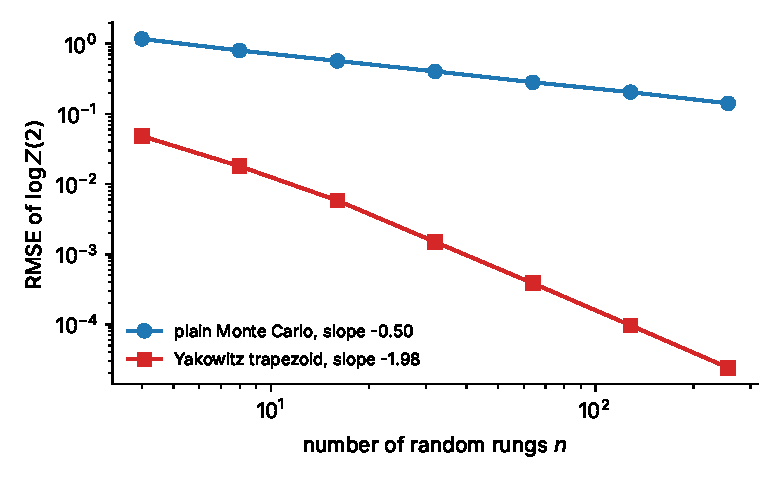
\includegraphics[width=0.85\textwidth]{figures/yakowitz_ti.pdf}
\caption[Yakowitz weighted Monte Carlo against plain Monte Carlo]{Root mean square error of $\log Z(2)$ by thermodynamic integration with $n$ random rungs. Plain Monte Carlo falls like $n^{-1/2}$; the trapezoid rule on the sorted rungs falls like $n^{-2}$, as the theory of Masry and Cambanis predicts.}
\label{fig:yak}
\end{figure}

A practical warning came out of the test. Our first run showed a rate of $n^{-1}$, not $n^{-2}$. The cause was a numerical defect in the integrand near $\gamma=0$, where a finite difference step crossed the origin. The weighted rule is only as good as the smoothness of the integrand, and a single jump costs a full order. This is useful in reverse: an observed rate below $n^{-2}$ is evidence of a jump in the integrand, which in thermodynamic integration means a first order phase transition or a numerical error.

\subsection{Where it helps, and where it does not}

The weighted rule helps whenever the random points are one dimensional and the integrand is smooth.
\begin{itemize}
\item Simulated tempering visits couplings at random. Sorting the visited couplings and applying the trapezoid rule to the measured mean actions gives a free energy with the Yakowitz rate in the quadrature, leaving only the Monte Carlo error of each mean.
\item Thorin densities and spectral integrals evaluated at sampled energies benefit in the same way.
\item The positive deconvolution above integrates a fitted measure against smooth kernels; sorted support points with trapezoid weights improve those integrals.
\end{itemize}
It does not help where the dominant error is not quadrature. In nested sampling the ordinates $X_i$ are not observed but estimated, with an error of order $\sqrt{H/N}$ in $\log Z$, and replacing rectangles by trapezoids in $X$ changed our estimates by only $0.005$ against a statistical error of $0.2$. Nor does it help in high dimensions directly: the rate rests on one dimensional spacings. The vertical identity of Section~\ref{ch:vertical} is what makes it relevant, by turning a high dimensional integral into a one dimensional one over likelihood ordinates or couplings.

\subsection{A connection with Euler Maclaurin}

The weighted rule is closely related to the sawtooth corrections in Stirling type expansions of $\log n!$ and to the Euler Maclaurin formula: the trapezoid rule on equally spaced points has error governed by Bernoulli numbers, and random spacings replace those constants by moments of exponential spacings.

\section*{Exercises}
\begin{enumerate}
\item Show that $\chi^2(\delta)$ is nondecreasing in $\delta$, and that the profile estimate $\hat\Delta$ is therefore well defined for any threshold $c$ for which the defining set is nonempty (this chapter, the support constrained profile).
\item Show that a sum of SU(2) elements is a nonnegative multiple of an SU(2) element, and derive the von Mises Fisher form of the link conditional. (Section~\ref{ch:latent})
\item Write out the slice sampler for $a_0$ with density proportional to $\sqrt{1-a_0^2}\,e^{\kappa a_0}$, and compare its acceptance with the Kennedy and Pendleton method for large $\kappa$. (Section~\ref{ch:latent})
\item Prove that the shrinkage factors in nested sampling are Beta$(N,1)$, and deduce that $-\log X_i$ is a sum of independent exponential variables with mean $1/N$. (Section~\ref{ch:latent})
\item Derive the torus formula $Z(\beta)=e^{-\beta P}\sum_nc_n(\beta)^P$ by integrating out links in the character expansion, and find the polynomial rate at which $Z(\beta)$ decays as $\beta\to\infty$. (Section~\ref{ch:latent})
\item Prove both identities $Z=\int_0^\infty T(y)\mathrm dy=\int_0^1\ell(s)\mathrm ds$. (Section~\ref{ch:vertical})
\item Show that $w\equiv1$ gives the harmonic mean estimator and explain its infinite variance in terms of the ordinate law. (Section~\ref{ch:vertical})
\item Show that $w(u)=au^{a-1}$ gives the power posterior, and derive the thermodynamic integration identity from it. (Section~\ref{ch:vertical})
\item For lattice gauge theory, write the default weight in terms of the density of states and explain why its importance function is independent of $\beta$. (Section~\ref{ch:vertical})
\item Show that uniform spacings have the law of independent exponential variables divided by their sum. (Section~\ref{ch:yakowitz})
\item Compute the mean square error of the weighted rule for $f(x)=x^2$ exactly and verify the $n^{-4}$ rate. (Section~\ref{ch:yakowitz})
\item Explain why the weighted rule with an integrand that has a jump has root mean square error of order $n^{-1}$, while a kink leaves the rate $n^{-2}$. (Section~\ref{ch:yakowitz})
\end{enumerate}
